\documentclass[aspectratio=169]{beamer}
\usepackage{xcolor}
\usepackage{multicol}
\usepackage{hyperref}
\usepackage{amsmath}
\usepackage{mhchem}
\usepackage{subcaption}
\usepackage{xparse}
\usepackage{physics}
\usepackage[mathscr]{euscript}  % \mathscr
\usepackage[style=verbose, backend=biber]{biblatex}
\usepackage{tikz}
\usetikzlibrary{shapes.geometric}

% Metadata of the presentation
\title{Phase Transitions in the Bose-Hubbard Model}
\subtitle{An in Depth Study of the Mott-Insulator to Superfluid Transition}
\author[DB]{Xeno De Vriendt, Robbe Brants}
\date{\today}


% Macro aimed at loading themes in different directories
\makeatletter
  \def\beamer@calltheme#1#2#3{%
    \def\beamer@themelist{#2}
    \@for\beamer@themename:=\beamer@themelist\do
    {\usepackage[{#1}]{\beamer@themelocation/#3\beamer@themename}}}

  \def\usefolder#1{
    \def\beamer@themelocation{#1}
  }
  \def\beamer@themelocation{}

% Load the UGent theme
\usefolder{./theme}
\usetheme[language=en,faculty=we,usecolors]{ugent}
\useinnertheme{ugent}
\useoutertheme{ugent}
\usecolortheme{ugent}
\usefonttheme{ugent}

% Path to images
\graphicspath{{./theme/}}

\bibliography{presentation.bib}


% Have this if you'd like section slides 
\AtBeginSection[]{
    \sectionframe
}

% \NewDocumentEnvironment{itemizewithimage}{ m b }{%
% \begin{center}%
%     \includegraphics[height=4cm,width=\textwidth,keepaspectratio]{#1}%
% \end{center}%
% \vfill%
% \begin{minipage}[t][3cm][t]{\textwidth}
%   \begin{itemize}%
%       #2
%   \end{itemize}%
% \end{minipage}
% }{%
% }
\definecolor{ugent_blue}{RGB}{30, 100, 200}
\renewcommand\emph[1]{\textcolor{ugent_blue}{\textbf{#1}}}

\begin{document}

\titleframe

\begin{frame}
  \frametitle{Importance of the Hubbard model: optical lattice containing ultra cold atoms}
  Making two coherent laser beams propagating in opposite directions interfere with each other.
    \begin{onlyenv}<1>
      \begin{figure}
        \includegraphics[scale=0.25]{../img/Optical-lattice-creation-a.png}
        \caption{Laser beam creates potential well \footcite{Greiner2008}.}
      \end{figure}
    \end{onlyenv}
    \begin{onlyenv}<2>
      \begin{figure}
        \includegraphics[scale=0.25]{../img/Optical-lattice-creation-a.png} \includegraphics[scale=0.25]{../img/Optical-lattice-creation-b.png}
        \caption{Interference causes standing waves \footnotemark[1].}
      \end{figure} 
    \end{onlyenv}
    \begin{onlyenv}<3>
      \begin{figure}
        \includegraphics[scale=0.25]{../img/Optical-lattice-creation-a.png} \includegraphics[scale=0.25]{../img/Optical-lattice-creation-b.png}\includegraphics[scale=0.25]{../img/Optical-lattice-creation-c.png}
        \caption{Four such lasers create a lattice \footnotemark[1].}
      \end{figure} 
    \end{onlyenv}
\end{frame}

\begin{frame}
  \frametitle{Optical lattices containing super cold atoms closely resemble condensed matter physics
  }
  \begin{onlyenv}<1>
    \begin{figure}
      \includegraphics[scale=0.4]{../img/real-crystal.png}
      \caption{Potential well created by attractive electrostatic force between the electrons (-) and the ions (+) forming the crystal \footnotemark[1].}
    \end{figure}
  \end{onlyenv}
  \begin{onlyenv}<2>
    \begin{figure}
      \includegraphics[scale=0.4]{../img/real-crystal.png} \\
      \includegraphics[scale=0.4]{../img/lattice.png}
      \caption{Simulated very well by an optical lattice \footnotemark[1].}
    \end{figure}
  \end{onlyenv}
\end{frame}

\begin{frame}
  \frametitle{Such lattices are indispensible in the study of different phases of matter}
  \begin{onlyenv}<1-3>
    \begin{columns}[T] % align columns
      \begin{column}{.48\textwidth}
        \begin{center}
          \includegraphics[scale=0.2]{../img/SF.png}
        \end{center}
      \end{column}%
      \hfill%
      \begin{column}{.48\textwidth}
        \begin{itemize}
          \item<2-> \textbf{Superfluid phase}\footnotemark[1]
          \item<3-> Potential for single particle excitations independent from number of particles 
        \end{itemize}
      \end{column}%
    \end{columns}
  \end{onlyenv}
  \begin{onlyenv}<4->
    \begin{columns}[T] % align columns
      \begin{column}{.48\textwidth}
        \begin{center}
          \includegraphics[scale=0.2]{../img/SF-MI.png}
        \end{center}
      \end{column}%
      \hfill%
      \begin{column}{.48\textwidth}
        \begin{itemize}
          \item<4-> \textbf{Superfluid phase}\footnotemark[1]
          \item<4-> Potential for single particle excitations independent from number of particles
          \item<4-> \textbf{Mott-insulator phase}\footnotemark[1]
          \item<5-> Strives for integer occupation in every potential well
        \end{itemize}
        \begin{alertblock}{Bose-Hubbard model}<6->
          Provides a relatively simple theoretical model to simulate these phenomena.
        \end{alertblock}
      \end{column}%
    \end{columns}
  \end{onlyenv}
\end{frame}

\begin{frame}
\frametitle{The bose-Hubbard Hamiltonian}
\begin{onlyenv}<1>
  \begin{equation}
    \hat{H} = \sum_{<i,j>} t_{ij}\hat{b}_i^\dagger \hat{b}_j + \frac{1}{2}\sum_i U_i\hat{b}_i^{\dagger 2} \hat{b}_i^{2} + \sum_i \omega_i \hat{b}_i^\dagger \hat{b}_i
  \end{equation}
  \begin{center}
    \includegraphics[scale=0.1]{../img/H.png}
  \end{center}
\end{onlyenv}
\begin{onlyenv}<2>
  \begin{equation}\tag{1}
    \hat{H} = \sum_{<i,j>} t_{ij}\hat{b}_i^\dagger \hat{b}_j + \frac{1}{2}\sum_i U_i\hat{b}_i^{\dagger 2} \hat{b}_i^{2} \color{blue}+ \sum_i \omega_i \hat{b}_i^\dagger \hat{b}_i
  \end{equation}
  \begin{center}
    \includegraphics[scale=0.1]{../img/omega.png}
  \end{center}
\end{onlyenv}
\begin{onlyenv}<3>
  \begin{equation}\tag{1}
    \hat{H} = \textcolor{green}{\sum_{<i,j>} t_{ij}\hat{b}_i^\dagger \hat{b}_j} + \frac{1}{2}\sum_i U_i\hat{b}_i^{\dagger 2} \hat{b}_i^{2} \textcolor{blue}{+ \sum_i \omega_i \hat{b}_i^\dagger \hat{b}_i}
  \end{equation}
  \begin{center}
    \includegraphics[scale=0.1]{../img/t.png}
  \end{center}
\end{onlyenv}
\begin{onlyenv}<4>
  \begin{equation}\tag{1}
    \hat{H} = \textcolor{green}{\sum_{<i,j>} t_{ij}\hat{b}_i^\dagger \hat{b}_j} \textcolor{violet}{+ \frac{1}{2}\sum_i U_i\hat{b}_i^{\dagger 2} \hat{b}_i^{2}} \textcolor{blue}{+ \sum_i \omega_i \hat{b}_i^\dagger \hat{b}_i}
  \end{equation}
  \begin{center}
    \includegraphics[scale=0.1]{../img/u.png}
  \end{center}
\end{onlyenv}
\end{frame}

\begin{frame}
  \frametitle{Studying phase transitions}
  \framesubtitle{Occupation connstraints and exact diagonalization}
  \begin{equation}
    \ket{\vb{c}} = \sum_{\vb{k}}c_{\vb{k}}\ket{\vb{k}}\thinspace ,
    \label{eq:fock_space}
  \end{equation}
  where the energy is given by
  \begin{equation}
    \hat{\mathcal{H}} \ket{\vb{c}} = E(\vb{c}) \ket{\vb{c}} \thinspace .
    \label{eq:FCI_energy}
  \end{equation}
  A \emph{constraint} can be added to this framework as a feature operator acting as a perturbation on the Hamiltonian, weighed by $\lambda$:
  \begin{equation} \label{eq:modified_hamiltonian}
    \hat{\mathcal{H}}_{\text{mod}}(\lambda) = \hat{\mathcal{H}} - \lambda \hat{m} \thinspace .
  \end{equation}
\end{frame}

\begin{frame}
  \frametitle{Occupation redistributions on a three site system...}
  \begin{onlyenv}<1>
    \begin{center}
      \includegraphics[scale=0.17]{../img/constraints.jpeg}
    \end{center}
  \end{onlyenv}
  \begin{onlyenv}<2>
    \begin{center}
      \includegraphics[scale=0.17]{../img/constraints2.jpeg}
    \end{center}
  \end{onlyenv}
  \begin{onlyenv}<3>
    \begin{center}
      \includegraphics[scale=0.17]{../img/constraints3.jpeg}
    \end{center}
  \end{onlyenv}
  \begin{onlyenv}<4>
    \begin{center}
      \includegraphics[scale=0.17]{../img/constraints4.jpeg}
    \end{center}
  \end{onlyenv}
\end{frame}

\begin{frame}
  \frametitle{... Give rise to Mott-Hubbard plateaus}
  \framesubtitle{in the strong correlation regime}
  \begin{center}
    \includegraphics[scale=0.3]{../img/BH-3in3-NvsMu.pdf}
  \end{center}
\end{frame}

\begin{frame}
  \frametitle{... Give rise to Mott-Hubbard plateaus and flat-planes}
  \framesubtitle{in the strong correlation regime}
  \begin{center}
    \begin{columns}[onlytextwidth]
      \begin{column}{0.5\textwidth}
        \begin{figure}[ht]
          \centering
          \includegraphics[scale=0.2]{../img/BH-3in3-NvsMu.pdf}
          \caption*{Mott-Hubbard plateaus.}
        \end{figure}
      \end{column}

      \begin{column}{0.5\textwidth}
        \begin{figure}[ht]
          \centering
          \includegraphics[scale=0.2]{../img/BH-3in3-EvsN.pdf}
          \caption*{Flat-plane conditions.}
        \end{figure}
      \end{column}
    \end{columns}
  \end{center}
\end{frame}

\begin{frame}
  \frametitle{Using exact diagonalization to model the complete phase diagram}
  \framesubtitle<2>{fails to close the single particle excitation gap}
  \begin{onlyenv}<1>
    \begin{align}
      \mu^+(L) &= E_0(L, N+1) - E_0(L, N) \thinspace ,\\
      \mu^-(L) &= E_0(L, N) - E_0(L, N-1) \thinspace , \\
      \Delta(L) &= \mu^+(L) - \mu^-(L)
    \end{align}
  \end{onlyenv}
  \begin{onlyenv}<2>
    \begin{center}
      \includegraphics[scale=0.3]{../img/Mott-Lobes-ED.pdf}
    \end{center}
  \end{onlyenv}
\end{frame}

\begin{frame}
  \frametitle{Moving on to bigger systems}
  \framesubtitle{Matrix product states}
  \begin{itemize}
    \item<1-> Any quantum state can be written as a matrix product state by subsequent singular value decompositions
  \end{itemize}
  \begin{onlyenv}<2->
    \begin{equation} \label{eq: SVD-graphic}
      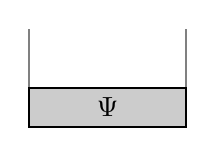
\begin{tikzpicture}[baseline={([yshift=-.5ex]current bounding box.center)}]
        \draw[gray, thick] (1,0) -- (1,1);
        \draw[gray, thick] (-1,0) -- (-1,1);
        \node (rect) at (0,0) [draw,thick,minimum width=2cm,minimum height=0.5cm, fill=black!20] {$\Psi$};
      \end{tikzpicture} = 
      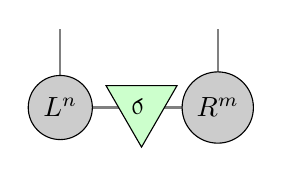
\begin{tikzpicture}[baseline={([yshift=-.5ex]current bounding box.center)}]
        \draw[gray, thick] (0,0) -- (0,1);
        \draw[gray, thick] (2,0) -- (2,1);
        \draw[gray, thick] (0,0) -- (2,0);
        \node[draw, circle, line cap=round, fill=black!20, minimum size=12] at (0,0) {$L^n$};
        \node[draw, isosceles triangle, isosceles triangle apex angle=60, rotate=30, line cap=round, fill=green!20, minimum size=12] at (1,0) { $\sigma$};
        \node[draw, circle, line cap=round, fill=black!20, minimum size=12] at (2,0) {$R^m$};
      \end{tikzpicture} \thinspace 
    \end{equation}
  \end{onlyenv}
  \begin{itemize}
    \item<3-> Where we introduce orthogonality relations
  \end{itemize}
  \begin{onlyenv}<3->
    \begin{equation} \label{eq:orthogonality-graphic}
        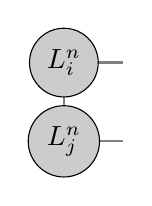
\begin{tikzpicture}[baseline={([yshift=-.5ex]current bounding box.center)}]
          \draw[gray, thick] (0,0) -- (0,-1);
          \draw[gray, thick] (0,0) -- (0.75,0);
          \draw[gray, thick] (0,-1) -- (0.75,-1);
          \node[draw, circle, line cap=round, fill=black!20, minimum size=12] at (0,0) {$L_i^n$};
          \node[draw, circle, line cap=round, fill=black!20, minimum size=12] at (0,-1) {$L_j^n$};
        \end{tikzpicture} = \delta_{ij} \thinspace , \qquad
        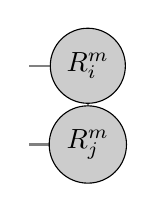
\begin{tikzpicture}[baseline={([yshift=-.5ex]current bounding box.center)}]
          \draw[gray, thick] (0,0) -- (0,-1);
          \draw[gray, thick] (0,0) -- (-0.75,0);
          \draw[gray, thick] (0,-1) -- (-0.75,-1);
          \node[draw, circle, line cap=round, fill=black!20, minimum size=12] at (0,0) {$R_i^m$};
          \node[draw, circle, line cap=round, fill=black!20, minimum size=12] at (0,-1) {$R_j^m$};
        \end{tikzpicture} = \delta_{ij}
    \end{equation}
  \end{onlyenv}
  \begin{itemize}
    \item<4> left, right and mixed canonical form 
  \end{itemize}
\end{frame}

\begin{frame}
  \frametitle{Moving on to bigger systems}
  \framesubtitle{Density matrix renormalization group}
  \begin{onlyenv}<2>
    \begin{equation}
      \min_\phi \bra{\psi - \phi}\ket{\psi - \phi} = \min_\phi [-2\bra{\phi}\ket{\psi} + \bra{\psi}\ket{\psi}] \thinspace 
    \end{equation}
  \end{onlyenv}
  \begin{onlyenv}<3>
    \begin{equation} 
      \bra{\phi}\ket{\psi} =
    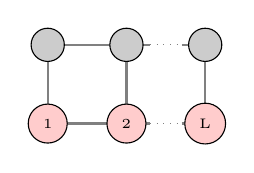
\begin{tikzpicture}[baseline={([yshift=-.5ex]current bounding box.center)}]
      % Open system
      \draw[gray, thick] (0,0) -- (0,-1);
      \draw[gray, thick] (1,0) -- (1,-1);
      \draw[gray, thick] (2,0) -- (2,-1);
  
      \draw[gray, thick] (0,0) -- (1.3,0);
      \draw[gray, dotted] (1.3,0) -- (1.7,0);
      \draw[gray, thick] (1.7,0) -- (2.0,0);
  
      \draw[gray, thick] (0,-1) -- (1.3,-1);
      \draw[gray, dotted] (1.3,-1) -- (1.7,-1);
      \draw[gray, thick] (1.7,-1) -- (2.0,-1);
  
      \node[draw, circle, line cap=round, fill=black!20, minimum size=12] at (0,0) {  };
      \node[draw, circle, line cap=round, fill=black!20, minimum size=12] at (1,0) {  };
      \node[draw, circle, line cap=round, fill=black!20, minimum size=12] at (2,0) {  };
  
      \node[draw, circle, line cap=round, fill=red!20] at (0,-1) {\tiny 1};
      \node[draw, circle, line cap=round, fill=red!20] at (1,-1) {\tiny 2};
      \node[draw, circle, line cap=round, fill=red!20] at (2,-1) {\tiny L};
    \end{tikzpicture} \thinspace , \qquad
    \bra{\psi}\ket{\psi} = 
    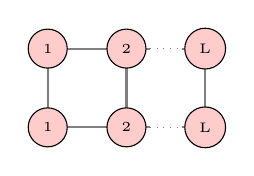
\begin{tikzpicture}[baseline={([yshift=-.5ex]current bounding box.center)}]
      % Open system
      \draw[gray, thick] (0,0) -- (0,-1);
      \draw[gray, thick] (1,0) -- (1,-1);
      \draw[gray, thick] (2,0) -- (2,-1);
  
      \draw[gray, thick] (0,0) -- (1.3,0);
      \draw[gray, dotted] (1.3,0) -- (1.7,0);
      \draw[gray, thick] (1.7,0) -- (2.0,0);
  
      \draw[gray, thick] (0,-1) -- (1.3,-1);
      \draw[gray, dotted] (1.3,-1) -- (1.7,-1);
      \draw[gray, thick] (1.7,-1) -- (2.0,-1);
  
      \node[draw, circle, line cap=round, fill=red!20] at (0,0) {\tiny 1};
      \node[draw, circle, line cap=round, fill=red!20] at (1,0) {\tiny 2};
      \node[draw, circle, line cap=round, fill=red!20] at (2,0) {\tiny L};
  
      \node[draw, circle, line cap=round, fill=red!20] at (0,-1) {\tiny 1};
      \node[draw, circle, line cap=round, fill=red!20] at (1,-1) {\tiny 2};
      \node[draw, circle, line cap=round, fill=red!20] at (2,-1) {\tiny L};    
    \end{tikzpicture} \thinspace 
  \end{equation}
  \end{onlyenv}
  \begin{onlyenv}<4>
    \begin{equation}\label{eq:gradient-1}
      \pderivative{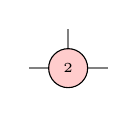
\begin{tikzpicture}
        \draw[gray, thick] (0,0) -- (1,0);
        \draw[gray, thick] (0.5,0) -- (0.5,0.5);
        \node[draw, circle, line cap=round, fill=red!20] at (0.5,0) {\tiny 2};
      \end{tikzpicture}} \left[ 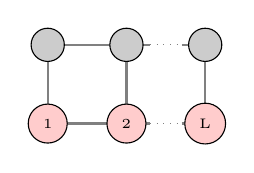
\begin{tikzpicture}[baseline={([yshift=-.5ex]current bounding box.center)}]
        % Open system
        \draw[gray, thick] (0,0) -- (0,-1);
        \draw[gray, thick] (1,0) -- (1,-1);
        \draw[gray, thick] (2,0) -- (2,-1);
    
        \draw[gray, thick] (0,0) -- (1.3,0);
        \draw[gray, dotted] (1.3,0) -- (1.7,0);
        \draw[gray, thick] (1.7,0) -- (2.0,0);
    
        \draw[gray, thick] (0,-1) -- (1.3,-1);
        \draw[gray, dotted] (1.3,-1) -- (1.7,-1);
        \draw[gray, thick] (1.7,-1) -- (2.0,-1);
    
        \node[draw, circle, line cap=round, fill=black!20, minimum size=12] at (0,0) {  };
        \node[draw, circle, line cap=round, fill=black!20, minimum size=12] at (1,0) {  };
        \node[draw, circle, line cap=round, fill=black!20, minimum size=12] at (2,0) {  };
    
        \node[draw, circle, line cap=round, fill=red!20] at (0,-1) {\tiny 1};
        \node[draw, circle, line cap=round, fill=red!20] at (1,-1) {\tiny 2};
        \node[draw, circle, line cap=round, fill=red!20] at (2,-1) {\tiny L};
      \end{tikzpicture} \right] = 
      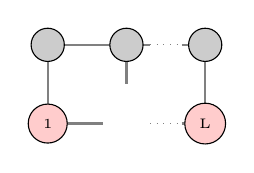
\begin{tikzpicture}[baseline={([yshift=-.5ex]current bounding box.center)}]
        % Open system
        \draw[gray, thick] (0,0) -- (0,-1);
        \draw[gray, thick] (1,0) -- (1,-0.5);
        \draw[gray, thick] (2,0) -- (2,-1);
    
        \draw[gray, thick] (0,0) -- (1.3,0);
        \draw[gray, dotted] (1.3,0) -- (1.7,0);
        \draw[gray, thick] (1.7,0) -- (2.0,0);
    
        \draw[gray, thick] (0,-1) -- (0.7,-1);
        \draw[gray, dotted] (1.3,-1) -- (1.7,-1);
        \draw[gray, thick] (1.7,-1) -- (2.0,-1);
    
        \node[draw, circle, line cap=round, fill=black!20, minimum size=12] at (0,0) {  };
        \node[draw, circle, line cap=round, fill=black!20, minimum size=12] at (1,0) {  };
        \node[draw, circle, line cap=round, fill=black!20, minimum size=12] at (2,0) {  };
    
        \node[draw, circle, line cap=round, fill=red!20] at (0,-1) {\tiny 1};
        \node[draw, circle, line cap=round, fill=red!20] at (2,-1) {\tiny L};
      \end{tikzpicture} \thinspace 
    \end{equation}
    \begin{equation}\label{eq:gradient-2}
      \pderivative{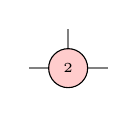
\begin{tikzpicture}
        \draw[gray, thick] (0,0) -- (1,0);
        \draw[gray, thick] (0.5,0) -- (0.5,0.5);
        \node[draw, circle, line cap=round, fill=red!20] at (0.5,0) {\tiny 2};
      \end{tikzpicture}} \left[ 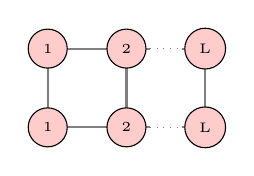
\begin{tikzpicture}[baseline={([yshift=-.5ex]current bounding box.center)}]
        % Open system
        \draw[gray, thick] (0,0) -- (0,-1);
        \draw[gray, thick] (1,0) -- (1,-1);
        \draw[gray, thick] (2,0) -- (2,-1);
    
        \draw[gray, thick] (0,0) -- (1.3,0);
        \draw[gray, dotted] (1.3,0) -- (1.7,0);
        \draw[gray, thick] (1.7,0) -- (2.0,0);
    
        \draw[gray, thick] (0,-1) -- (1.3,-1);
        \draw[gray, dotted] (1.3,-1) -- (1.7,-1);
        \draw[gray, thick] (1.7,-1) -- (2.0,-1);
    
        \node[draw, circle, line cap=round, fill=red!20] at (0,0) {\tiny 1};
        \node[draw, circle, line cap=round, fill=red!20] at (1,0) {\tiny 2};
        \node[draw, circle, line cap=round, fill=red!20] at (2,0) {\tiny L};
    
        \node[draw, circle, line cap=round, fill=red!20] at (0,-1) {\tiny 1};
        \node[draw, circle, line cap=round, fill=red!20] at (1,-1) {\tiny 2};
        \node[draw, circle, line cap=round, fill=red!20] at (2,-1) {\tiny L};    
      \end{tikzpicture} \right] = 2 \left[
      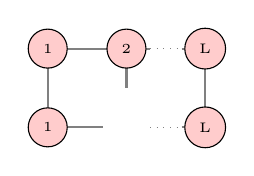
\begin{tikzpicture}[baseline={([yshift=-.5ex]current bounding box.center)}]
        % Open system
        \draw[gray, thick] (0,0) -- (0,-1);
        \draw[gray, thick] (1,0) -- (1,-0.5);
        \draw[gray, thick] (2,0) -- (2,-1);
    
        \draw[gray, thick] (0,0) -- (1.3,0);
        \draw[gray, dotted] (1.3,0) -- (1.7,0);
        \draw[gray, thick] (1.7,0) -- (2.0,0);
    
        \draw[gray, thick] (0,-1) -- (0.7,-1);
        \draw[gray, dotted] (1.3,-1) -- (1.7,-1);
        \draw[gray, thick] (1.7,-1) -- (2.0,-1);
    
        \node[draw, circle, line cap=round, fill=red!20] at (0,0) {\tiny 1};
        \node[draw, circle, line cap=round, fill=red!20] at (1,0) {\tiny 2};
        \node[draw, circle, line cap=round, fill=red!20] at (2,0) {\tiny L};
    
        \node[draw, circle, line cap=round, fill=red!20] at (0,-1) {\tiny 1};
        \node[draw, circle, line cap=round, fill=red!20] at (2,-1) {\tiny L};
      \end{tikzpicture} \right] \thinspace 
    \end{equation}
  \end{onlyenv}
  \begin{onlyenv}<5-7>
    \begin{itemize}
      \item Consider
    \end{itemize}
    \begin{equation}
      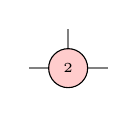
\begin{tikzpicture}[baseline={([yshift=-.5ex]current bounding box.center)}]
        \draw[gray, thick] (0,0) -- (1,0);
        \draw[gray, thick] (0.5,0) -- (0.5,0.5);
        \node[draw, circle, line cap=round, fill=red!20] at (0.5,0) {\tiny 2};
      \end{tikzpicture} = A^n_{ij} \equiv a[nij] 
    \end{equation}
  \end{onlyenv}
  \begin{onlyenv}<6-7>
    \begin{itemize}
      \item Then
    \end{itemize}
    \begin{equation}\label{eq:gradient-1-as-tensor}
      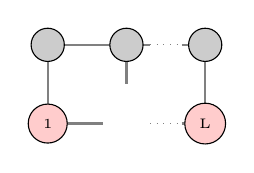
\begin{tikzpicture}[baseline={([yshift=-.5ex]current bounding box.center)}]
        % Open system
        \draw[gray, thick] (0,0) -- (0,-1);
        \draw[gray, thick] (1,0) -- (1,-0.5);
        \draw[gray, thick] (2,0) -- (2,-1);
    
        \draw[gray, thick] (0,0) -- (1.3,0);
        \draw[gray, dotted] (1.3,0) -- (1.7,0);
        \draw[gray, thick] (1.7,0) -- (2.0,0);
    
        \draw[gray, thick] (0,-1) -- (0.7,-1);
        \draw[gray, dotted] (1.3,-1) -- (1.7,-1);
        \draw[gray, thick] (1.7,-1) -- (2.0,-1);
    
        \node[draw, circle, line cap=round, fill=black!20, minimum size=12] at (0,0) {  };
        \node[draw, circle, line cap=round, fill=black!20, minimum size=12] at (1,0) {  };
        \node[draw, circle, line cap=round, fill=black!20, minimum size=12] at (2,0) {  };
    
        \node[draw, circle, line cap=round, fill=red!20] at (0,-1) {\tiny 1};
        \node[draw, circle, line cap=round, fill=red!20] at (2,-1) {\tiny L};
      \end{tikzpicture} = b^T
    \end{equation}
  \end{onlyenv}
  \begin{onlyenv}<7>
    \begin{itemize}
      \item which leads to
    \end{itemize}
    \begin{equation}
      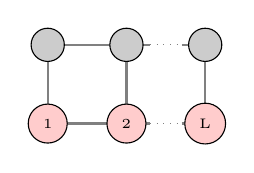
\begin{tikzpicture}[baseline={([yshift=-.5ex]current bounding box.center)}]
        % Open system
        \draw[gray, thick] (0,0) -- (0,-1);
        \draw[gray, thick] (1,0) -- (1,-1);
        \draw[gray, thick] (2,0) -- (2,-1);
    
        \draw[gray, thick] (0,0) -- (1.3,0);
        \draw[gray, dotted] (1.3,0) -- (1.7,0);
        \draw[gray, thick] (1.7,0) -- (2.0,0);
    
        \draw[gray, thick] (0,-1) -- (1.3,-1);
        \draw[gray, dotted] (1.3,-1) -- (1.7,-1);
        \draw[gray, thick] (1.7,-1) -- (2.0,-1);
    
        \node[draw, circle, line cap=round, fill=black!20, minimum size=12] at (0,0) {  };
        \node[draw, circle, line cap=round, fill=black!20, minimum size=12] at (1,0) {  };
        \node[draw, circle, line cap=round, fill=black!20, minimum size=12] at (2,0) {  };
    
        \node[draw, circle, line cap=round, fill=red!20] at (0,-1) {\tiny 1};
        \node[draw, circle, line cap=round, fill=red!20] at (1,-1) {\tiny 2};
        \node[draw, circle, line cap=round, fill=red!20] at (2,-1) {\tiny L};
      \end{tikzpicture} = b^T a \thinspace , \qquad
      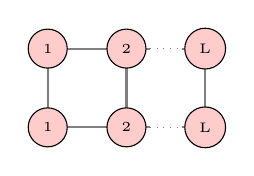
\begin{tikzpicture}[baseline={([yshift=-.5ex]current bounding box.center)}]
        % Open system
        \draw[gray, thick] (0,0) -- (0,-1);
        \draw[gray, thick] (1,0) -- (1,-1);
        \draw[gray, thick] (2,0) -- (2,-1);
      
        \draw[gray, thick] (0,0) -- (1.3,0);
        \draw[gray, dotted] (1.3,0) -- (1.7,0);
        \draw[gray, thick] (1.7,0) -- (2.0,0);
      
        \draw[gray, thick] (0,-1) -- (1.3,-1);
        \draw[gray, dotted] (1.3,-1) -- (1.7,-1);
        \draw[gray, thick] (1.7,-1) -- (2.0,-1);
      
        \node[draw, circle, line cap=round, fill=red!20] at (0,0) {\tiny 1};
        \node[draw, circle, line cap=round, fill=red!20] at (1,0) {\tiny 2};
        \node[draw, circle, line cap=round, fill=red!20] at (2,0) {\tiny L};
      
        \node[draw, circle, line cap=round, fill=red!20] at (0,-1) {\tiny 1};
        \node[draw, circle, line cap=round, fill=red!20] at (1,-1) {\tiny 2};
        \node[draw, circle, line cap=round, fill=red!20] at (2,-1) {\tiny L};    
      \end{tikzpicture} = a^T M a \thinspace
    \end{equation}
  \end{onlyenv}
  \begin{onlyenv}<8->
    \begin{itemize}
      \item with
    \end{itemize}
       \begin{equation}
        M = 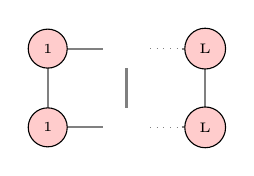
\begin{tikzpicture}[baseline={([yshift=-.5ex]current bounding box.center)}]
        % Open system
        \draw[gray, thick] (0,0) -- (0,-1);
        \draw[gray, thick] (1,-0.25) -- (1,-0.75);
        \draw[gray, thick] (2,0) -- (2,-1);
    
        \draw[gray, thick] (0,0) -- (0.7,0);
        \draw[gray, dotted] (1.3,0) -- (1.7,0);
        \draw[gray, thick] (1.7,0) -- (2.0,0);
    
        \draw[gray, thick] (0,-1) -- (0.7,-1);
        \draw[gray, dotted] (1.3,-1) -- (1.7,-1);
        \draw[gray, thick] (1.7,-1) -- (2.0,-1);
    
        \node[draw, circle, line cap=round, fill=red!20] at (0,0) {\tiny 1};
        \node[draw, circle, line cap=round, fill=red!20] at (2,0) {\tiny L};
    
        \node[draw, circle, line cap=round, fill=red!20] at (0,-1) {\tiny 1};
        \node[draw, circle, line cap=round, fill=red!20] at (2,-1) {\tiny L};
      \end{tikzpicture} 
    \end{equation}
  \end{onlyenv}
  \begin{onlyenv}<9->
    \begin{itemize}
      \item Which, due to eq. (9), reduces the optimization problem to 
    \end{itemize}
    \begin{equation}
      Ma = b \rightarrow a = b
    \end{equation}
  \end{onlyenv}
\end{frame}

\begin{frame}
  \frametitle{DMRG can model the Mott-insulator - superfluid phase diagram}
  \framesubtitle{for a system of 128 sites}
  \begin{center}
    \includegraphics[scale=0.3]{../img/Mott-Lobes.pdf}
  \end{center}
\end{frame}

\begin{frame}
  \frametitle{The superfluid phase compensates uniformly for impurities}
  \begin{columns}[onlytextwidth]
    \begin{column}{0.5\textwidth}
      \begin{figure}[ht]
        \centering
        \includegraphics[scale=0.2]{../img/Density-profiles-MI.pdf}
        \caption*{Mott-insulator.}
      \end{figure}
    \end{column}
    \begin{column}{0.5\textwidth}
      \begin{figure}[ht]
        \centering
        \includegraphics[scale=0.2]{../img/Density-profiles-SF.pdf}
        \caption*{Superfluid.}
      \end{figure}
    \end{column}
  \end{columns}
\end{frame}

\begin{frame}
  \frametitle{Fractional filling of the system in the superfluid phase induces density waves}
  \framesubtitle<3>{And impurities cause interference}
  \begin{onlyenv}<1-2>
    \begin{center}
      \includegraphics[scale=0.22]{../img/Density-profiles-fractional-density.pdf}
    \end{center}
  \end{onlyenv}
  \begin{onlyenv}<2>
    \begin{equation}
      \langle n(r)n(0) \rangle_w \sim (\rho r)^{-2/K} \cos(2\pi\rho r) \thinspace .
      \label{eq:waves}
    \end{equation}
  \end{onlyenv}
  \begin{onlyenv}<3>
    \begin{columns}[onlytextwidth]
      \begin{column}{0.5\textwidth}
        \begin{figure}[ht]
          \centering
          \includegraphics[scale=0.2]{../img/Density-profiles-fractional-density.pdf}
          \caption*{Without impurity.}
        \end{figure}
      \end{column}
      \begin{column}{0.5\textwidth}
        \begin{figure}[ht]
          \centering
          \includegraphics[scale=0.2]{../img/Density-profiles-fractional-impurity.pdf}
          \caption*{With impurity.}
        \end{figure}
      \end{column}
    \end{columns}
  \end{onlyenv}
\end{frame}


\begin{frame}
  \frametitle<1-2>{Correlation function decays exponentially in the Mott-insulator...}
  \begin{onlyenv}<1-2>
    \begin{center}
      \includegraphics[scale=0.22]{../img/Correlations-MI1.pdf}
    \end{center}
  \end{onlyenv}
  \begin{onlyenv}<2>
    \begin{equation}\label{eq:correlation decay}
      \Gamma(r) = \langle b^\dagger(r)b(0)\rangle \thinspace .
    \end{equation}
  \end{onlyenv}
  \frametitle<3>{...and algebraically in the superfluid phase}
  \begin{onlyenv}<3>
    \begin{columns}[onlytextwidth]
      \begin{column}{0.5\textwidth}
        \begin{figure}[ht]
          \centering
          \includegraphics[scale=0.2]{../img/Correlations-SF1.pdf}
          \caption*{SF with integer occupation.}
        \end{figure}
      \end{column}
      \begin{column}{0.5\textwidth}
        \begin{figure}[ht]
          \centering
          \includegraphics[scale=0.2]{../img/Correlations-SF2.pdf}
          \caption*{SF with fractional occupation.}
        \end{figure}
      \end{column}
    \end{columns}
    \begin{equation}
      r^{-K/2}
    \end{equation}
  \end{onlyenv}
\end{frame}

\begin{frame}
  \frametitle<1>{Bond dimension influences the decay function}
  \begin{onlyenv}<1>
    \begin{figure}[ht]
      \centering
      \includegraphics[scale=0.3]{../img/Correlations-bonds.pdf}
    \end{figure}
  \end{onlyenv}
  \frametitle<2>{Bond dimension \emph{and finite size effects} influences the decay function}
  \begin{onlyenv}<2>
    \begin{columns}[onlytextwidth]
      \begin{column}{0.5\textwidth}
        \begin{figure}[ht]
          \centering
          \includegraphics[scale=0.2]{../img/Correlations-bonds.pdf}
          \caption*{Decay with respect to bond dimension.}
        \end{figure}
      \end{column}

      \begin{column}{0.5\textwidth}
        \begin{figure}[ht]
          \centering
          \includegraphics[scale=0.2]{../img/Correlations-lengths.pdf}
          \caption*{Decay with respect to system size.}
        \end{figure}
      \end{column}
    \end{columns}
  \end{onlyenv}
\end{frame}

\begin{frame}
  \frametitle{Decay function indicates presence of critical point: The Berezinskii-Kosterlitz-Thouless transition}
  \framesubtitle{The Mott-insulator phase}
  \begin{onlyenv}<1->
    \begin{center}
      \includegraphics[scale=0.22]{../img/Correlations-length-values.pdf}
    \end{center}
  \end{onlyenv}
  \begin{onlyenv}<1>
    \begin{equation}
      \exp(\frac{-r}{\xi})
    \end{equation}
  \end{onlyenv}
  \begin{onlyenv}<2>
    \begin{equation}
      t/U \approx 0.3
    \end{equation}
  \end{onlyenv}
\end{frame}

\begin{frame}
  \frametitle{Decay function indicates presence of critical point: The Berezinskii-Kosterlitz-Thouless transition}
  \framesubtitle{The superfluid phase}
  \begin{onlyenv}<1->
    \begin{center}
      \includegraphics[scale=0.2]{../img/Correlations-K-values.pdf}
    \end{center}
  \end{onlyenv}
  \begin{onlyenv}<1>
    \begin{equation}
      r^{-K/2}
    \end{equation}
  \end{onlyenv}
  \begin{onlyenv}<2->
    \begin{itemize}
      \item<2-> $\rho \rightarrow n$, with $n$ an integer value 
      \item<3-> $\rho = \frac{31}{32}$
      \item<4-> $t_c \approx 0.33$
    \end{itemize}
  \end{onlyenv}
\end{frame}

\begin{frame}
  \frametitle{Conclusions}
  \begin{columns}[onlytextwidth]
    \begin{column}{0.33\textwidth}
      \begin{onlyenv}<2->
        \begin{figure}[ht]
          \centering
          \includegraphics[height=2cm, width=\textwidth,keepaspectratio]{../img/BH-3in3-NvsMu.pdf}
          \caption*{Mott-Hubbard plateaus.}
        \end{figure}   
      \end{onlyenv}

      \begin{onlyenv}<5->
        \begin{figure}[ht]
          \centering
          \includegraphics[height=2cm, width=\textwidth,keepaspectratio]{../img/Density-profiles-fractional-density.pdf}
          \caption*{Fractional occupations induce density waves.}
        \end{figure}   
      \end{onlyenv}
    \end{column}

    \begin{column}{0.33\textwidth}
      \begin{onlyenv}<3->
        \begin{figure}[ht]
          \centering
          \includegraphics[height=2cm, width=\textwidth,keepaspectratio]{../img/Mott-Lobes.pdf}
          \caption*{Full Phase diagram with DMRG.}
        \end{figure}   
      \end{onlyenv}

      \begin{onlyenv}<6->
        \begin{figure}[ht]
          \centering
          \includegraphics[height=2cm, width=\textwidth,keepaspectratio]{../img/Correlations-lengths.pdf}
          \caption*{Finite size effects affect decay.}
        \end{figure}   
      \end{onlyenv}
    \end{column}

    \begin{column}{0.33\textwidth}
      \begin{onlyenv}<4->
        \begin{figure}[ht]
          \centering
          \includegraphics[height=2cm, width=\textwidth,keepaspectratio]{../img/Density-profiles-SF.pdf}
          \caption*{$\omega_i$ affect SF homogeneously.}
        \end{figure}   
      \end{onlyenv}

      \begin{onlyenv}<7->
        \begin{figure}[ht]
          \centering
          \includegraphics[height=2cm, width=\textwidth,keepaspectratio]{../img/Correlations-K-values.pdf}
          \caption*{Decay indicates critical point.}
        \end{figure}   
      \end{onlyenv}
    \end{column}
  \end{columns}
\end{frame}
 
  

\end{document}
